\documentclass[a4paper,12pt]{article}
\usepackage[utf8]{inputenc}
\usepackage[T1]{fontenc}
\usepackage[hungarian]{babel}
\usepackage{graphicx}
\usepackage{geometry}
\geometry{a4paper,
		     tmargin = 35mm, 
		     lmargin = 25mm,
		     rmargin = 30mm,
		     bmargin = 30mm}
\usepackage{mathtools}
\usepackage{amsmath}
\usepackage{color}
\usepackage{setspace}
\usepackage{amsmath,amssymb}
\usepackage{float}


\usepackage{indentfirst}
\usepackage{subfig}

\renewcommand\thesection{\Roman{section}}

\begin{document}

\linespread{1.2}

\begin{titlepage}

	\centering
	
\includegraphics[width=0.66\textwidth]{elte.jpg}\par\vspace{1cm}
	{\scshape\LARGE ELTE TTK \par}
	\vspace{3cm}
	{\scshape\Large Mag-mágneses rezonancia vizsgálata\par}
	\vspace{1cm}
	{\large\itshape Olar Alex\par}
	\vspace{3cm}
	{\large 2018 \par}
	
\end{titlepage}

\begin{abstract}

\par Mag-mágneses rezonancia során a mágneses térbe helyezett atomok rezonancia szerű elnyelést produkálnak. A labor célja ennek a jelenségnek a lehető legpontosabb kimérése volt az adott eszközökkel. 


\end{abstract}

\vfill

\tableofcontents

\newpage

\section{Elméleti összefoglaló, mérési eszközök}

\par A mag-mágneses rezonancia jelenségét a következőképpen vizsgáltuk: állandó, homogén mágneses térbe helyeztük a mintát, amit egy áramgenerátor szolgáltatott. Egy feszültség generátor egy másik, sokkal kisebb fluxusú mágneses teret adott ehhez hozzá, ezzel vittünk be gerjesztést a rendszerbe a rezonancia-jelenség vizsgálatához. Ez utóbbi váltóáramú egységről jött.

\par A közel homogén mágneses tér előállításához azért használtunk áramgenerátort, mivel az sokkal pontosbannan működik, mint egy feszültséggenerátor, így az inhomogenitásokat jobban elkerülhetőek. A moduláló térnél az amplitudó nem igazán számított ( amíg elhanyagolhatóan kicsi, lényegében mindegy, hogy mekkore ), így ott a feszültséggenerátor megfelelt erre a célre.

\par Továbbá felhasználtuk azt, hogy a mintát egy rezgőkörhöz kötve helyeztük a homogén mágneses térbe. Ezt használjük gerjesztésre, és mivel oszcillátor kapcsolásba van kötve, így mérésre is használható, hiszen az amplitúdó csökkenése így jelzi az abszorpciót. Ezért is kellett a koax-kábel kimenetét ehhez a gerjesztő dobozra kötni.

\par A mágneses tér mérésére egy ballisztikus galvanométert használtunk. Ezen egy osztás $3.35 ~mT \pm 0.01 ~mT$-nak felelt meg. Amikor a galvanométer mérőrúdját kirántottuk a mágneses térből, így hirtelen fluxusváltozást keltve, az analóg mutató $2.9 ~s$ relaxációs idővel kilengett, így nagy bizonyossággal leolvasható volt a mért tér érték háromszori validálás után.

\section{Mérési feladatok, kiértékelés}

\par Először is a mérés szempontjából fontos lenne megállapítani, hogy mennyire pontosan homogén a mágneses tér. Én függőleges irányban mértem ki a galvanométerrel a mágneses teret, ekkor a következő eredményeket kaptam.

\begin{center}
\begin{tabular}{|c|c|}
\hline
Magasság [$cm$] & Oszcilloszkóp egység \\
\hline
3.7 & 0.6 \\
\hline
3.2 & 0.8 \\
\hline
2.2 & 0.8 \\
\hline
5.5 & 0.7 \\
\hline
5.7 & 0.8 \\
\hline
7.1 & 0.6 \\
\hline
\end{tabular}
\end{center}

\par Az oszcilloszkópon azt vizsgáltuk, hogy az adott áramerősségen és frekvencián megjelenő abszorpciós csúcs helyzete mennyivel mozdul el a mintát mozgatva. A magasság/mélység mérését a plexilapok segítségével mértek a két mágnespofa közé felülről belógatva az egyiket. A hosszmérés hibája $\pm 2 ~mm$, míg az oszcilloszkópon leolvasott értékek hiába $0.05$ osztás körül volt. Lényegében ezek nem fontosak, hiszen ennél jóval nagyobb hibát pordukál az, hogy a függőleges mozgatás közben kicsit oldalra kimozdul a minta, hiszen vízszintesen közel sem annyira homogén a tér. Felső becslést adva a hibára, itt az csúcs legnagyobb elmozdulása $0.2$-es volt, ha a módusztól való eltérést vesszük alapul. Ennél biztosan kisebb a hibája a mágneses mezőnek, mivel ezzel felülbecslést végeztem.
\par Korábban lemértük, hogy az oszcilloszkóp kijelzőjén 1 beosztós $0.3 \%$-os eltérésnek felelet meg adott $f$ frekvenciánál, így mivel $B ~ f$, a mágneses térnek is, maximum $\delta B = 0.6 \%$-os relatív hibája lehet függőleges irányban.

\subsection{ A proton g-faktora}

\par Rázgálicos vízmintával különböző mágneses tereknél is vizsgáltuk a frekvenciát, ezen adatokat táblázatba szedve, valamint egy szemléltető ábra

\begin{center}
\begin{tabular}{|c|c|c|c|c|}
\hline
Gerjesztő frekvencia [MHz] & f [MHz] & Áramgen. & I [A] & Galvanométer \\
\hline
8.5 & 8.496 & 782 & 2.42 & 61 \\
\hline
8 & 8.325 & 766 & 2.37 & 60.5 \\
\hline
7.5 & 7.705 & 685 & 2.12 & 56 \\
\hline
7 & 7.285 & 626.5 & 1.94 & 53 \\
\hline
7 & 7.155 & 610 & 1.89 & 52 \\
\hline
6.5 & 6.754 & 623.5 & 1.93 & 49 \\
\hline
6 & 6.167 & 566 & 1.74 & 44.5 \\
\hline
5.5 & 5.641 & 514 & 1.57 & 41.5 \\
\hline
5 & 5.087 & 445.5 & 1.38 & 37 \\
\hline
4.5 & 4.515 & 373 & 1.15 & 33.5 \\
\hline
4 & 4.064 & 324 & 1 & 30 \\
\hline
3.5 & 3.675 & 284.5 & 0.87 & 27 \\
\hline
\end{tabular}
\end{center}

\begin{figure}[!h]
\centering
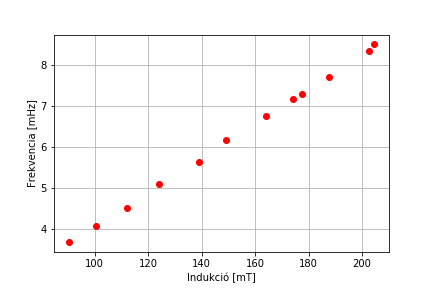
\includegraphics[width=0.85\textwidth]{indukcio-freki.png}
\end{figure}

\begin{figure}[!h]
\centering
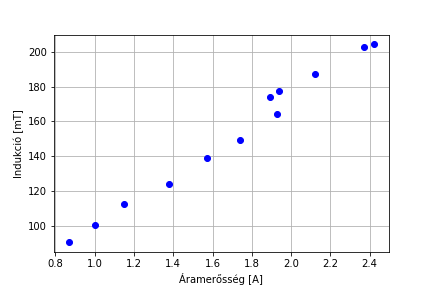
\includegraphics[width=0.85\textwidth]{./adatok/hiszterezis.png}
\label{Hiszeterézis}
\end{figure}

\par Ezek közül én az illesztést a 4.-8. sorokban lévő adatokra végeztem. További hibalehetőség volt, hogy a homogén mágneses tér időben nem teljesen állandó, így a mérés ideje alatt szintén változik egy kicsit, főként az áramköri elemek melegedésétől bekövetkező ellenállás változás miatt. Ezt szintén lemértük, hasonló módon, mint az inhomogenitásnál a csúcs elmozulásából származtattunk $0.18\%$-os relatív hibát, így a mágneses tér homogenitása 

\begin{equation*}
	\delta B = 0.78 ~\%
\end{equation*}

\par Fontos megjegyezni, hogy a galvanométer $3.35 \pm 0.01 ~mT/\text{osztás}$-ra volt valaidálva, de ez a hiba, csak szisztematikus, nem statisztikus hibaként jelenik meg, így figyelmen kívül hagytam és csak a végén adtam hozzá.

\par A frekvencia pontos mérésének is van több okból is hibája. Egyrészt a pontosság csak 4 jegyig jegyezhető, így $\Delta f = \pm 0.5 kHz$ a leolvasás hibája. Az időmérés hibáját egy rosszabb minőségű kvarcórával becsülve arra jutottunk, hogy a leolvasás hibájánal az több nagyságrenddel kisebb, így elhanyagolható. 

\par Így a proton g-faktorát az adataim alapján

\begin{center}
\begin{tabular}{|c|c|c|c|}
\hline
Frekvencia [MHz] & $\Delta$f [kHz] & Indukció [mT] & $\Delta$ B [mT] \\
\hline
7.155 & 0.5 & 174.2 & 1.34 \\
\hline
6.754 & 0.5 & 164.15 & 1.28 \\
\hline
6.167 & 0.5 & 149.08 & 1.16 \\
\hline
5.641 & 0.5 & 139.03 & 1.08 \\
\hline
\end{tabular}
\end{center}

\par Ezekre az adatokra origón átmenő egyenest illesztettem, amiből a proton giromágneses faktora:

\begin{equation*}
g_{p} = 5.389 \pm 0.120
\end{equation*}

\begin{center}
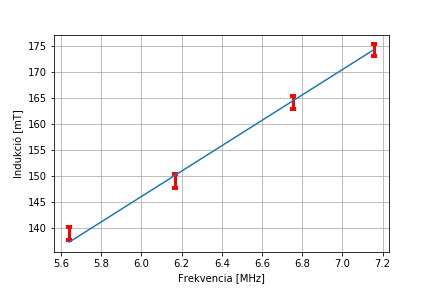
\includegraphics[width=0.75\textwidth]{./egyenes.png}
\end{center}

\par Ahol az illesztés meredeksége $(24.352 \pm 0.090) \cdot 10^{-9} ~\frac{T}{Hz}$ volt és ebből számoltam vissza, majd hozzáadtam a galvanométer kalibrációs hibáját.

\subsection{ g-faktorok aránya, proton és fluor}

\par Méréseink alapján

\begin{center}
\begin{tabular}{|c|c|} \hline
proton [MHz] & fluor [MHz] \\ \hline
5.920 $\pm$ 0.001 &	5.569 $\pm$ 0.001 \\ \hline
7.150 $\pm$ 0.001 &	6.726 $\pm$ 0.001 \\ \hline
\end{tabular}
\end{center}

\par Ahol a frekvencia mérésének hibáját a csúcs szélességéből $\pm 0.001 ~MHz$-nek becsültem mindkét esetben. Innen $\frac{g_{fluor}}{g_{proton}} \approx 0.9407$, ami jól közelíti az irodalmi értéket. A hiba csak a harmadik tizedesjegy után változtat, így mindenképpen kisebb a hiba, mint $5\%$-ék. 

\end{document}